\expandafter\ifx\csname ifdraft\endcsname\relax
 \begin{document}
\fi

\section{結果}

\subsection{実験時条件}

実験は各プロトコル別日に行った.実験時の条件を表\ref{tb:light_experiment}と表\ref{tb:hard_experiment}に示す.
なお,体重あたり酸素摂取量に使用される体重は,各プロトコル実験の直前に測定した.

\begin{table}[H]
  \begin{center}
  \caption{低強度プロトコル}
  \label{tb:light_experiment}
    \begin{tabular}{|l|l|}
      \hline
      実験日 & 2021/01/24 \\ \hline
      開始時刻 & 18:21:54 \\ \hline
      体重 & 55.0kg \\ \hline
      気温(平均) & 12.99℃ \\ \hline
      大気圧(平均) & 1021.76hPa \\ \hline
      飽和水蒸気圧(平均) & 14.97hPa \\ \hline
      STPD係数(平均) & 0.95 \\ \hline
    \end{tabular}
  \end{center}
\end{table}

\begin{table}[H]
  \begin{center}
  \caption{高強度プロトコル}
  \label{tb:hard_experiment}
    \begin{tabular}{|l|l|}
      \hline
      実験日 & 2021/01/25 \\ \hline
      開始時刻 & 10:32:46 \\ \hline
      体重 & 55.0kg \\ \hline
      気温(平均) & 18.92℃ \\ \hline
      大気圧(平均) & 1027.19 \\ \hline
      飽和水蒸気圧(平均) & 21.88hPa \\ \hline
      STPD係数(平均) & 0.93 \\ \hline
    \end{tabular}
  \end{center}
\end{table}

\subsection{実験結果}

図\ref{fig:light_hard_vo2},図\ref{fig:light_vo2_power},図\ref{fig:light_vo2_hr},図\ref{fig:hard_vo2_power},図\ref{fig:hard_vo2_hr}に実験結果のグラフを示す.凡例は各グラフの下部に示した.なお,凡例中のlightは低強度プロトコル,hardは高強度プロトコルを指す.

\subsubsection{低強度プロトコルと高強度プロトコルにおけるVO2}

\begin{figure}[H]
  \begin{center}
    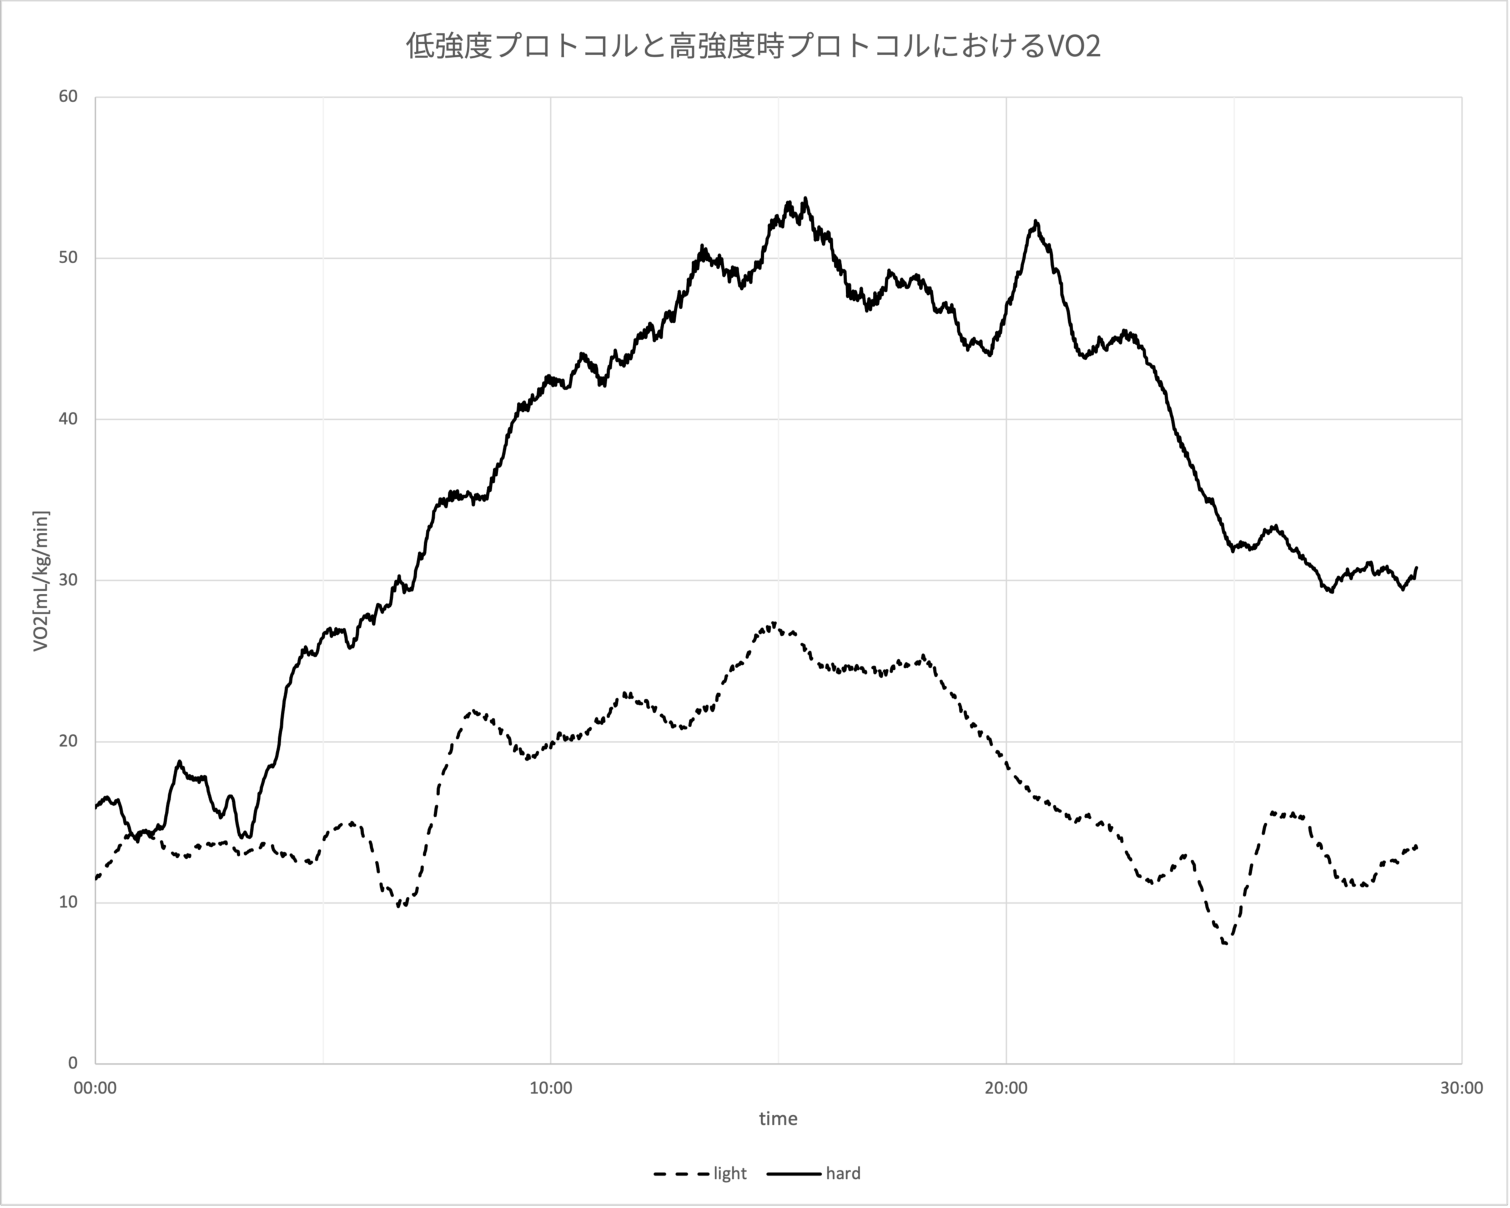
\includegraphics[width=12cm]{fig/light_hard_vo2}
    \caption{低強度プロトコルと高強度プロトコルにおけるVO2}
    \label{fig:light_hard_vo2}
  \end{center}
\end{figure}

低強度と高強度における酸素摂取量の変化(図\ref{fig:light_hard_vo2})を見ると,高強度において,低強度よりも酸素摂取量が大きくなっているのが分かる.また,開始6分時点に0Wから70Wに漸増する低強度と,開始3分時点に40Wから70Wに漸増する設定パワーによる酸素摂取量の増加のタイミングの違いが確認できる.低強度,高強度いずれの場合でもその後3分ごとに30Wずつ漸増していくが,最初の1分程度では低強度と高強度で同等の割合で増加を見せるのに対し,以降の増加の割合は設定パワーが高い高強度では低強度よりも大きくなっていることが確認できる.

酸素摂取量のピーク位置を見ると,低強度,高強度いずれの場合においても,酸素摂取量の最大値位置は15分付近で一致していることが分かる.

\subsubsection{低強度プロトコルにおけるVO2とパワー}

\begin{figure}[H]
  \begin{center}
    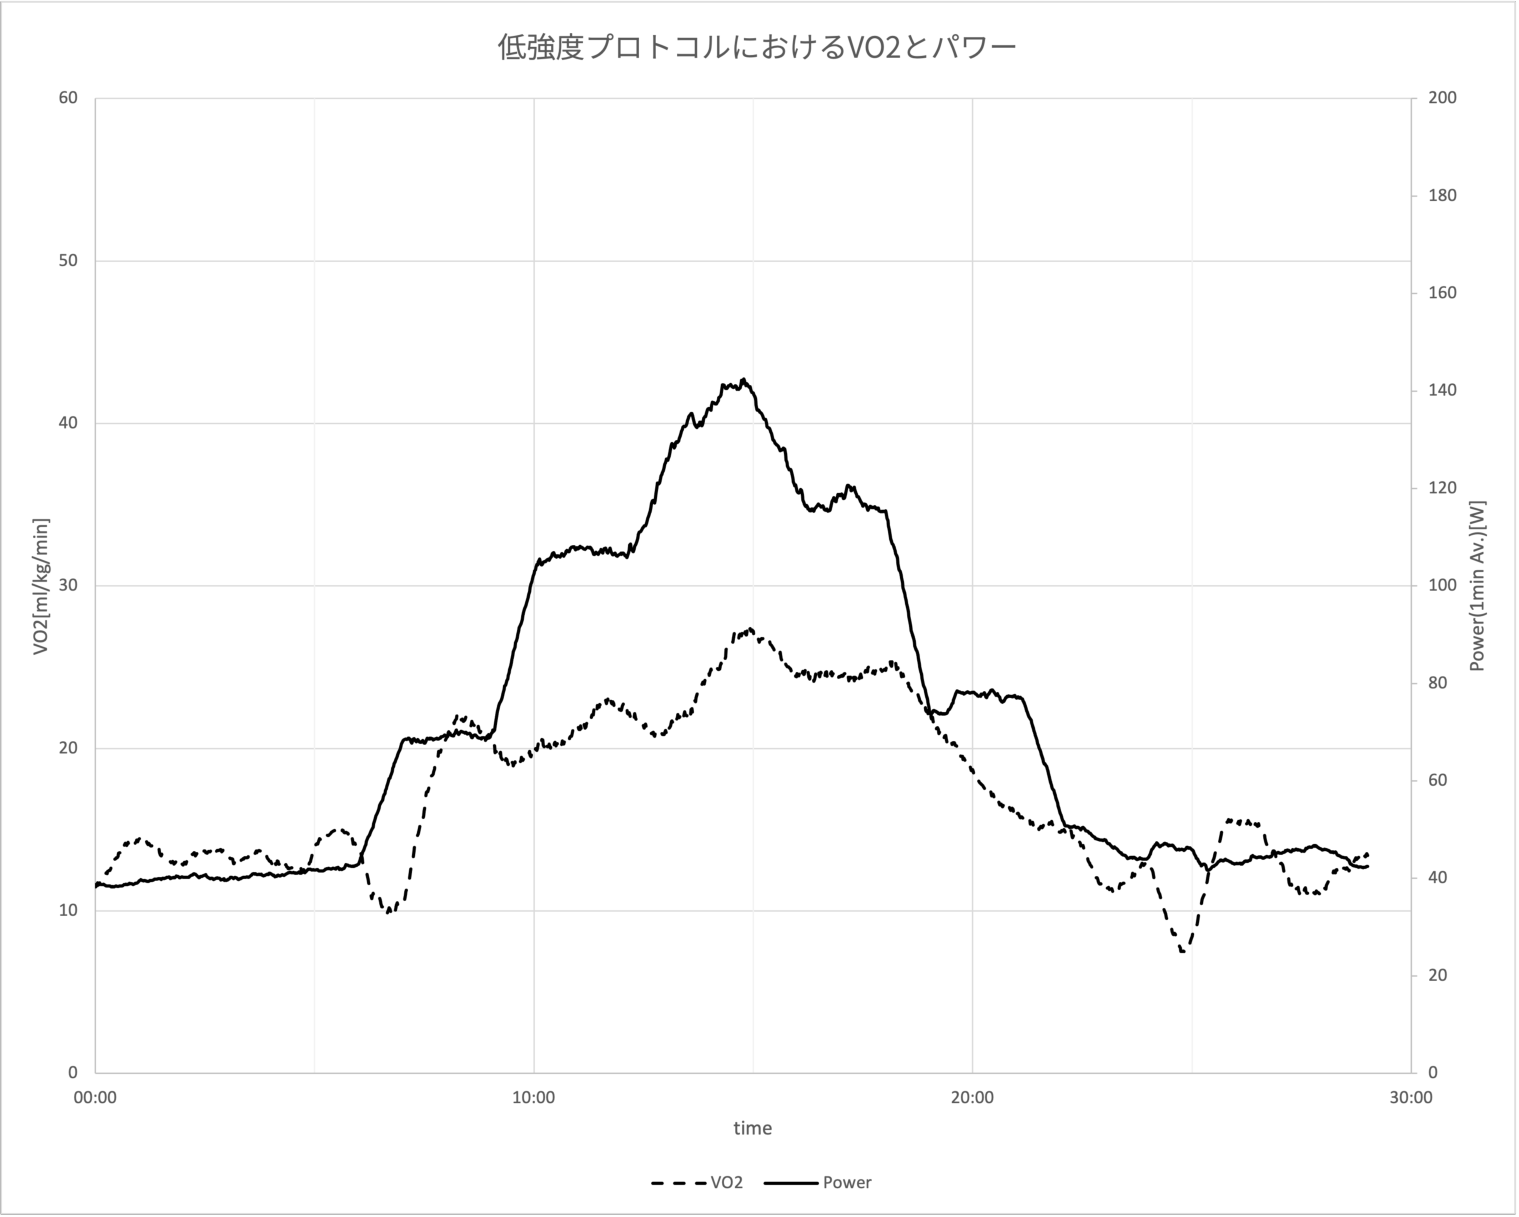
\includegraphics[width=12cm]{fig/light_vo2_power}
    \caption{低強度プロトコルにおけるVO2とパワー}
    \label{fig:light_vo2_power}
  \end{center}
\end{figure}

低強度における酸素摂取量とパワーの比較(図\ref{fig:light_vo2_power})では,負荷の漸増によって増加し15分時点で最大となった酸素摂取量が,漸減を始める15分時点以降でも増加時と同じような波形で減少しているのが分かる.

ピーク位置を見ると,酸素摂取量とパワーの最大値位置は15分付近で一致していることが分かる.

\subsubsection{低強度プロトコルにおけるVO2と心拍数}

\begin{figure}[H]
  \begin{center}
    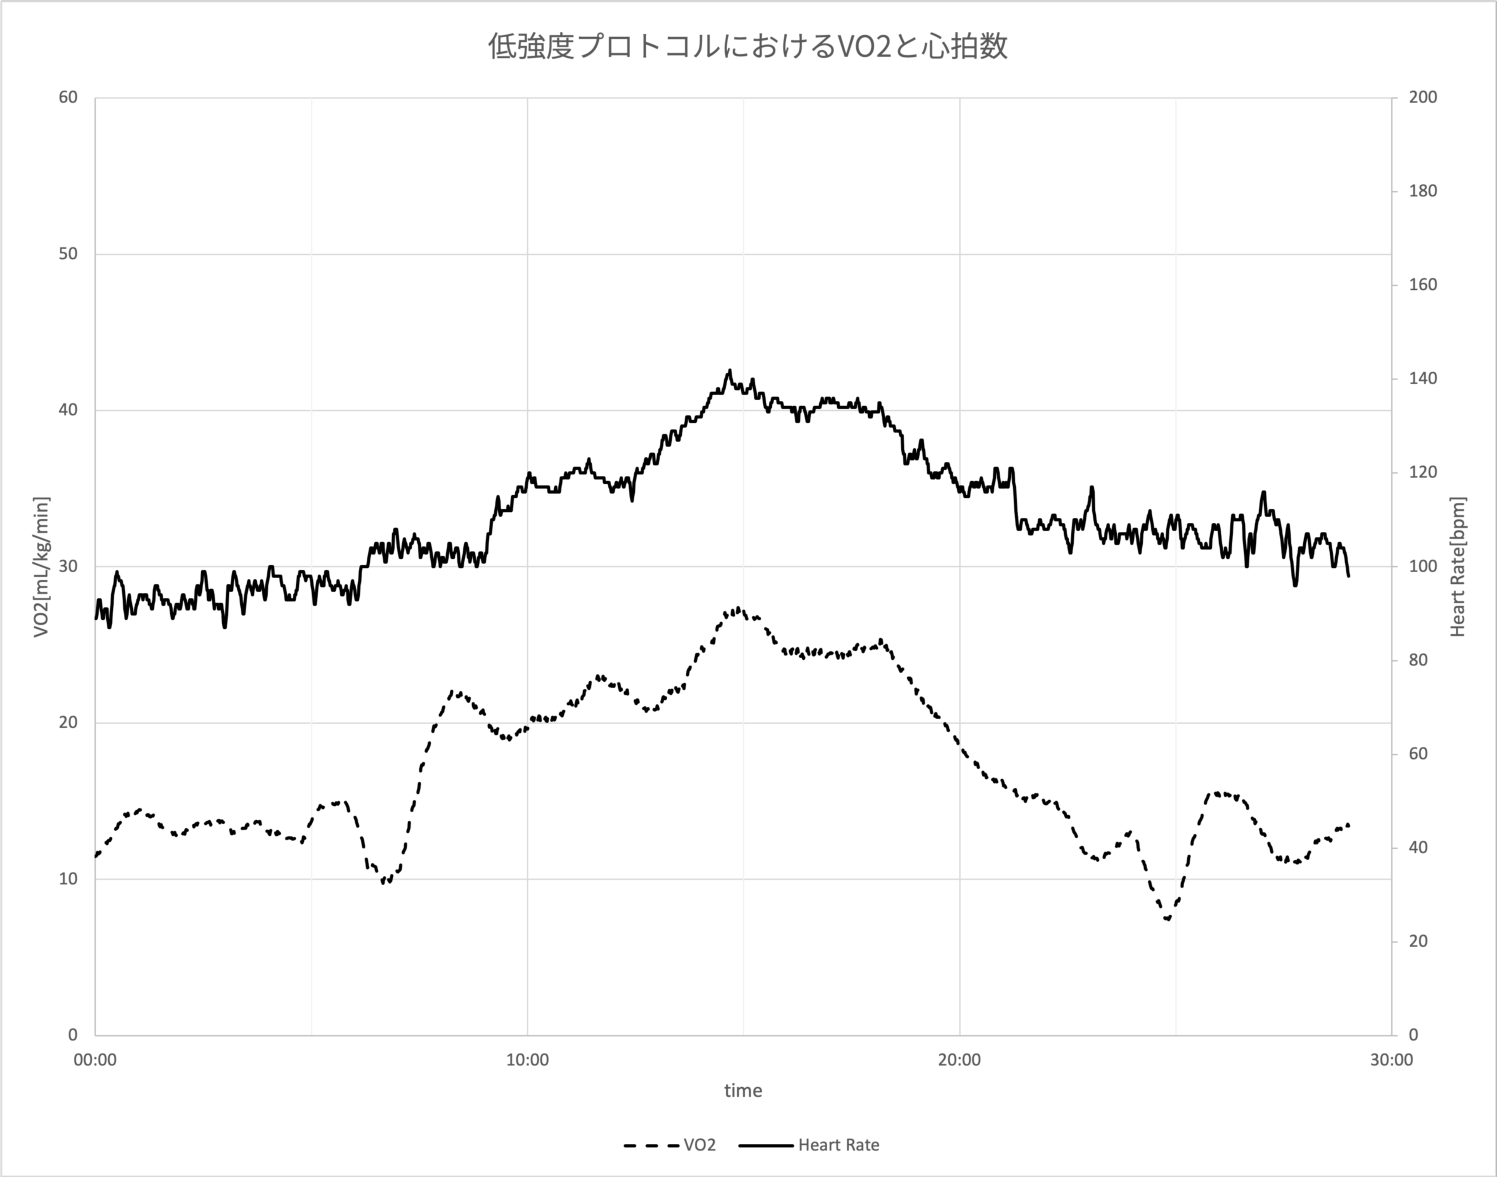
\includegraphics[width=12cm]{fig/light_vo2_hr}
    \caption{低強度プロトコルにおけるVO2と心拍数}
    \label{fig:light_vo2_hr}
  \end{center}
\end{figure}

低強度における酸素摂取量と心拍数の比較(図\ref{fig:light_vo2_hr})において,ピーク位置を見ると,酸素摂取量と心拍数の最大値位置は15分付近で一致していることが分かる.

\subsubsection{高強度プロトコルにおけるVO2とパワー}

\begin{figure}[H]
  \begin{center}
    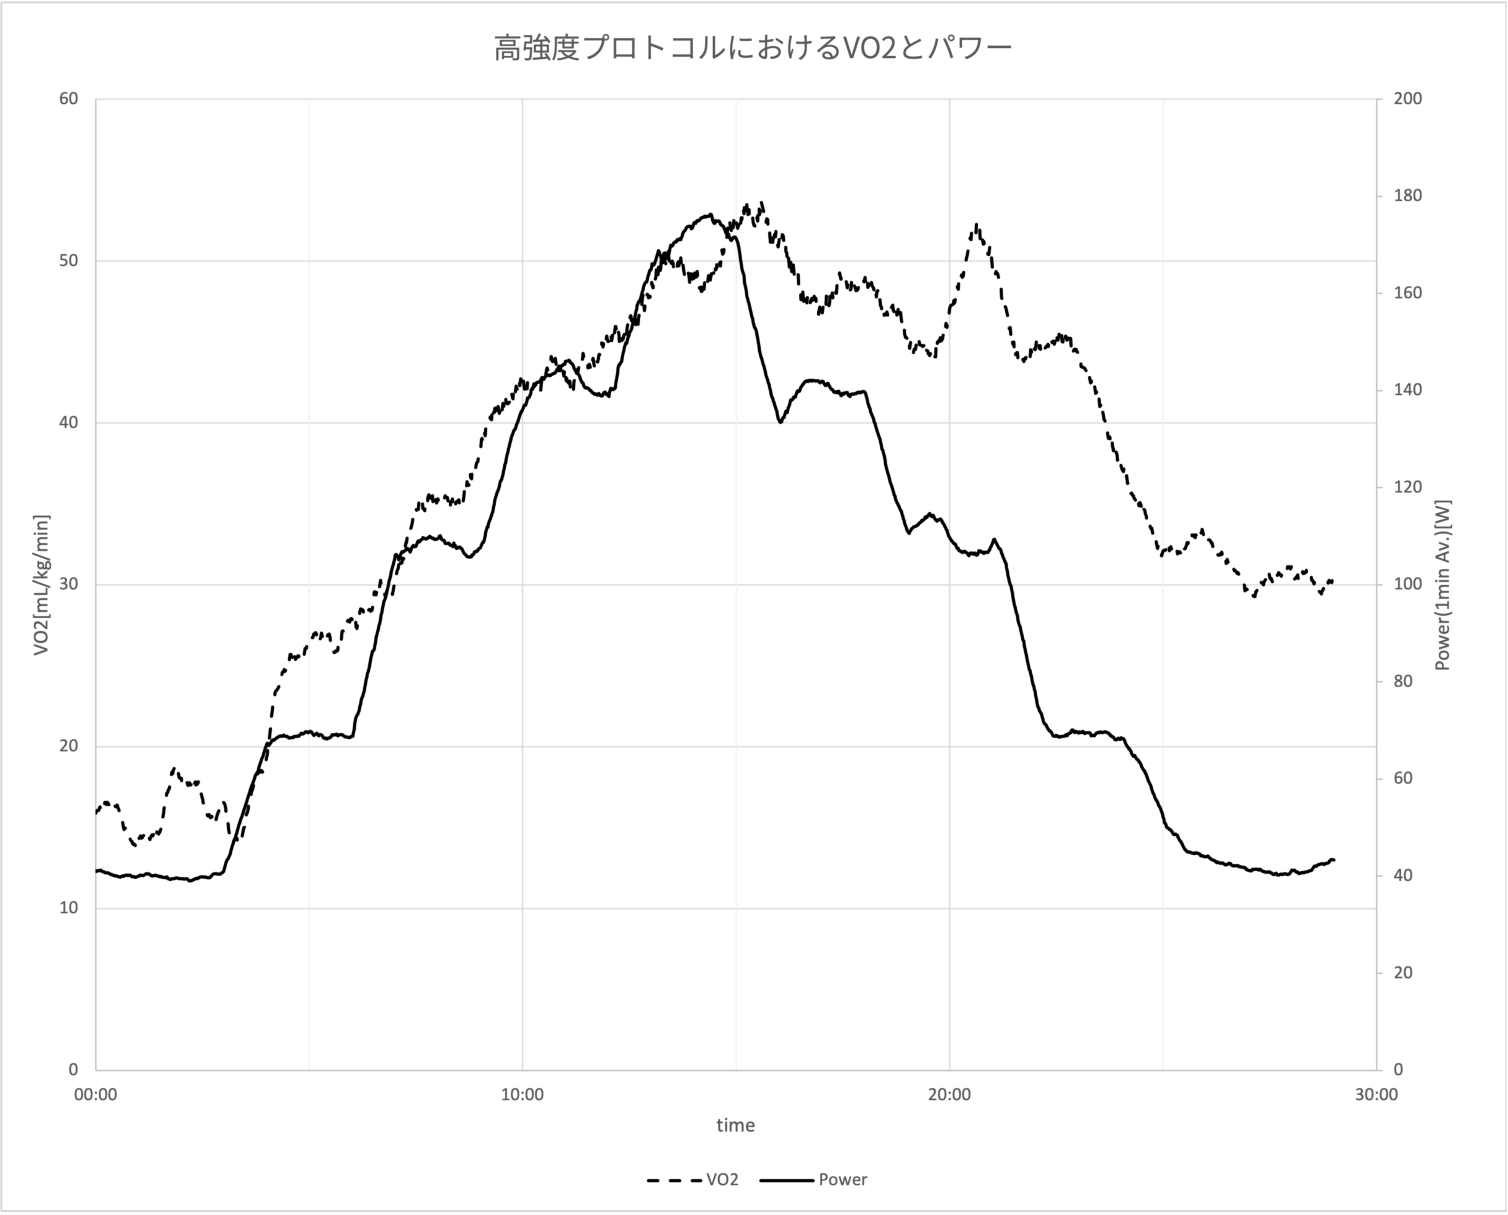
\includegraphics[width=12cm]{fig/hard_vo2_power}
    \caption{高強度プロトコルにおけるVO2とパワー}
    \label{fig:hard_vo2_power}
  \end{center}
\end{figure}

低強度における酸素摂取量とパワーの比較では,負荷の漸増,漸減を行った際に,酸素摂取量は増加時と同様の傾向で減少していく様子が見られた(図\ref{fig:light_vo2_power}).一方で,高強度における酸素摂取量とパワーの比較(図\ref{fig:hard_vo2_power})では,負荷を漸増していく15分時点までは酸素摂取量と同様の傾向で増加していくが,漸減を始める15分時点以降はパワーの波形を遅れてなぞるように減少していることが分かる.

ピーク位置を見ると,酸素摂取量とパワーの最大値位置は15分付近で一致していることが分かる.

\subsubsection{高強度プロトコルにおけるVO2と心拍数}

\begin{figure}[H]
  \begin{center}
    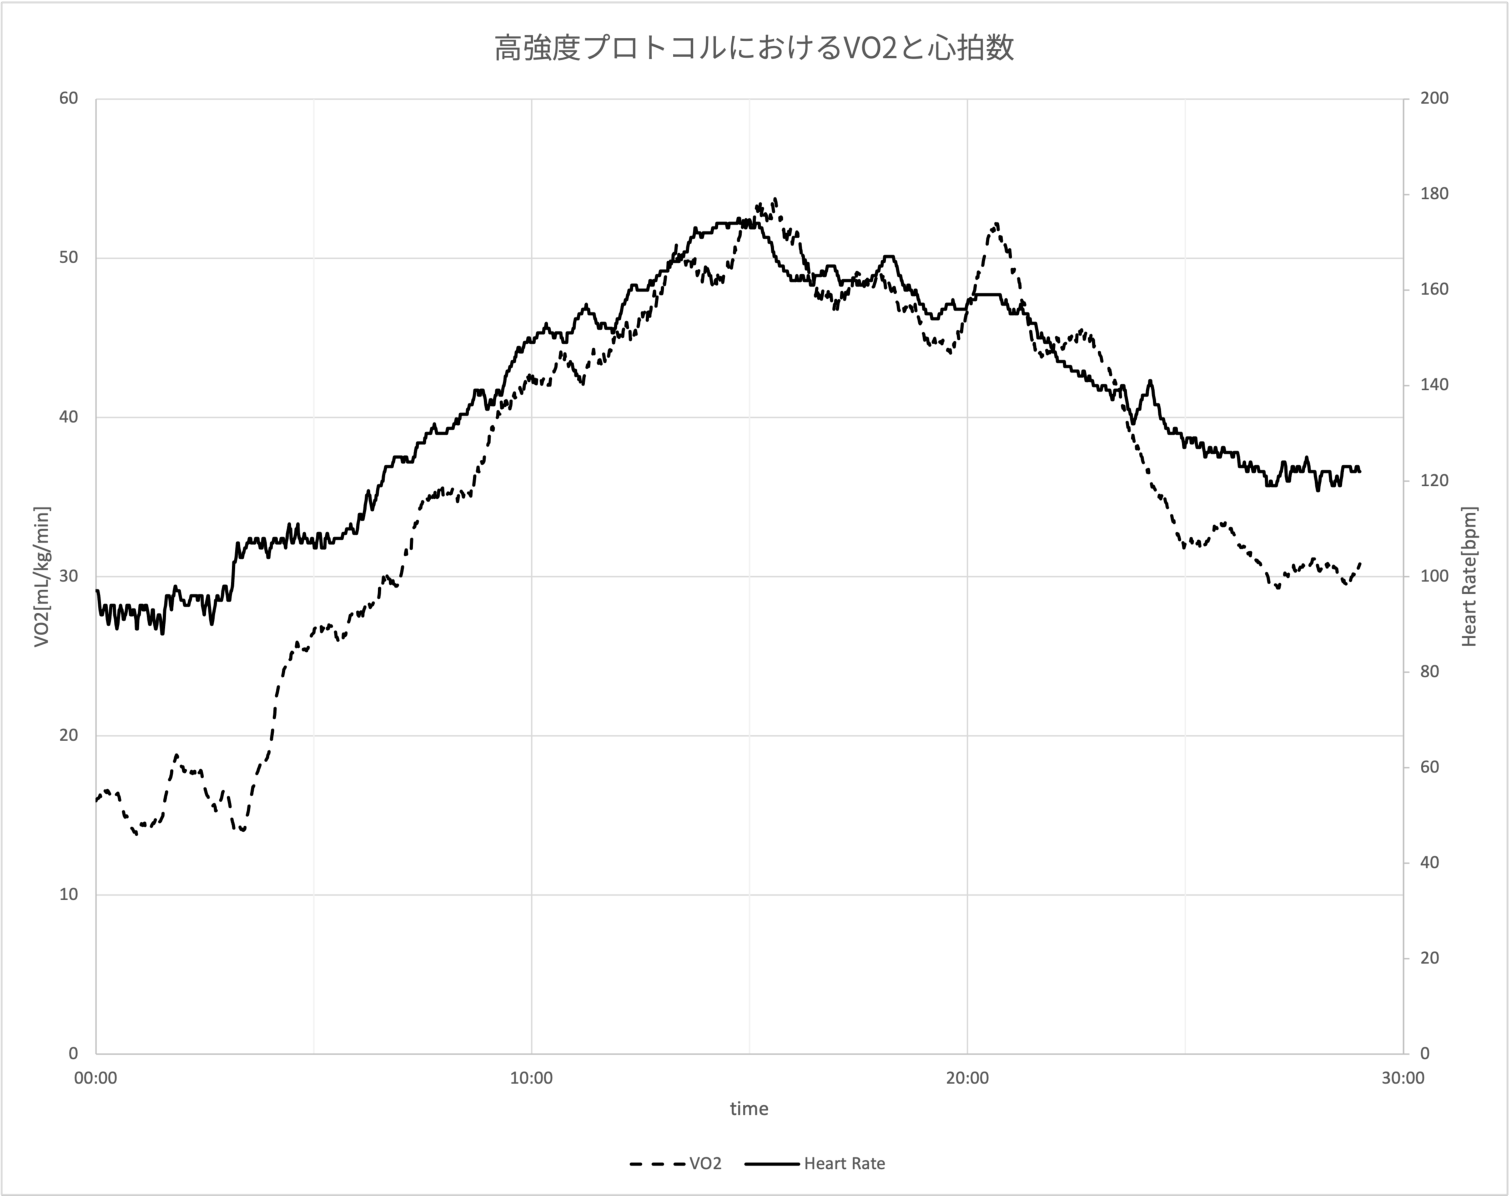
\includegraphics[width=12cm]{fig/hard_vo2_hr}
    \caption{高強度プロトコルにおけるVO2と心拍数}
    \label{fig:hard_vo2_hr}
  \end{center}
\end{figure}

高強度プロトコルにおける酸素摂取量と心拍数の比較(図\ref{fig:hard_vo2_hr})では,高強度における酸素摂取量とパワーの比較(図\ref{fig:hard_vo2_power})で酸素摂取量の変化に見られたような,負荷前漸増時の心拍数の増加の比べて負荷漸減時の心拍数の減少が緩やかになる傾向が見られる.

ピーク位置を見ると,酸素摂取量と心拍数の最大値位置は15分付近で一致していることが分かる.

\expandafter\ifx\csname ifdraft\endcsname\relax
  \end{document}
\fi
